\def\PageLayout{single-no-print}
\def\DocLanguage{en}
\def\PackagesIncludeTikz{yes}
\def\PackagesIncludeBib{yes}

%%% Different page dimensions used on thesis
\def\PageLayoutSingle{single}
\def\PageLayoutSingleNoPrint{single-no-print}
\def\PageLayoutDouble{double}
\def\PageLayoutDoubleNoPrint{double-no-print}



%% Single page print
\ifx\PageLayout\PageLayoutSingle
\documentclass[a4paper,oneside,12pt]{report}
\setlength\textwidth{145mm}
\setlength\textheight{251mm}
\setlength\oddsidemargin{15mm}
\setlength\evensidemargin{15mm}
\setlength\topmargin{-0.4in}
\setlength\headsep{10mm}
\setlength\headheight{0mm}
\let\openright=\clearpage
\fi

%% Double page print
\ifx\PageLayout\PageLayoutDouble
% \documentclass[12pt,a4paper,twoside,openright]{report} % chapter will always start on the right side
\documentclass[12pt,a4paper,twoside]{report}
\setlength\textwidth{145mm}
\setlength\textheight{251mm}
\setlength\oddsidemargin{14.2mm}
\setlength\evensidemargin{0mm}
\setlength\topmargin{-0.4in}
\setlength\headsep{10mm}
\setlength\headheight{0mm}
\let\openright=\clearpage
% \let\openright=\cleardoublepage
\fi

%% Double page without space left for binding
\ifx\PageLayout\PageLayoutDoubleNoPrint
% \documentclass[12pt,a4paper,twoside,openright]{report} % chapter will always start on the right side
\documentclass[12pt,a4paper,twoside]{report}
\setlength\textwidth{145mm}
\setlength\textheight{251mm}
\setlength\oddsidemargin{9mm}
\setlength\evensidemargin{9mm}
\setlength\topmargin{-0.4in}
\setlength\headsep{10mm}
\setlength\headheight{0mm}
\let\openright=\clearpage
% \let\openright=\cleardoublepage
\fi

%% Single page without space left for binding
\ifx\PageLayout\PageLayoutSingleNoPrint
\documentclass[12pt,a4paper]{report}
\setlength\textwidth{145mm}
\setlength\textheight{251mm}
\setlength\oddsidemargin{9mm}
\setlength\evensidemargin{9mm}
\setlength\topmargin{-0.4in}
\setlength\headsep{10mm}
\setlength\headheight{0mm}
\let\openright=\clearpage

\fi




\def\LangCS{cs}
\def\LangEN{en}
\def\ConfirmExpr{yes}




%%% TiKz
% Memoize package needs to be loaded as soon as possible, in beamer even before document declaration
\ifx\PackagesIncludeTikz\ConfirmExpr
	\usepackage{memoize}
	\usepackage{collargs}
	\usepackage{tikz}
	\usepackage{tikz-cd}
	\usepackage{circuitikz}
	\mmzset{memo dir=memoize}
	\mmzset{auto={circuitikz}{memoize}}
	\mmzset{auto={tikzcdi}{memoize, verbatim}}
	\mmzset{auto={tikzpicture}{memoize, verbatim}}

	\usetikzlibrary{calc}
	\usetikzlibrary{fadings}
	\usetikzlibrary{shapes.geometric, arrows, positioning}

	\tikzstyle{layerheader} = [rectangle, minimum width=3cm, minimum height=1cm, text centered, draw=black, fill=gray!30]
	\tikzstyle{startstop} = [ellipse, minimum width=3cm, minimum height=1cm, text centered, draw=black, fill=red!30]
	\tikzstyle{process} = [rectangle, minimum width=3cm, minimum height=1cm, text centered, draw=black, fill=blue!20]
	\tikzstyle{decision} = [diamond, minimum width=2.5cm, minimum height=1cm, text centered, draw=black, fill=green!20]
	\tikzstyle{arrow} = [thick,->,>=stealth]
\fi




\ifx\DocLanguage\LangCS
	\usepackage[czech]{babel}
	\babelprovide[transforms = oneletter.nobreak]{czech} % non break on single letter words in czech
\else
	\usepackage[english]{babel}
\fi


\usepackage[T1]{fontenc}
\usepackage[utf8]{inputenc}
\usepackage{lmodern,textcomp}

\usepackage[a-2u]{pdfx}         % adding metadata to pdf with .xmpdata file
\usepackage{graphicx}						% inserting pictures
\usepackage{caption}						%	captions of figures
\usepackage{subcaption} 				% multiple figures in one figure environment
\usepackage{hyperref} 					% handling of hypertext
\usepackage{tabularx}           % table environment
\usepackage{xcolor,colortbl}    % more options for colors
\usepackage{textpos}            % more precise control over positioning of elements
\usepackage{longtable}          % longtable environment to enable multipage tables
\usepackage{fancyhdr}						% custom header and footer
\usepackage{xurl}								% extension to url handeling, allows linebreaks in urls and more special characters
\usepackage{enumitem}           % more options for labeling lists
\usepackage{multicol}           % simplest environment to achieve multiple columns

%%% Math packages
\usepackage{pgfplots}           % graphs
\usepackage{amsmath}						% extension for math
\usepackage{amsthm}							% environment for lemmas, proofs, theorems, etc.
\usepackage{amssymb} 						% math symbols
\usepackage{mathrsfs}  	        % math symbols
\usepackage{mathabx}						% math symbols
\usepackage{mathrsfs} 					% Fancy italic used to denote Hilbert spaces and such
\usepackage{bbm} 							  % blackboard variants of computer Modern fonts useful for number groups, mean value notation
\usepackage{esint} 						  % adds more integrals
\usepackage{accents} 						% multiple mathematical accents
\usepackage{arcs} 							% arcs over and under words
\usepackage{steinmetz} 					% Steinmetz notation for complex numbers
\usepackage{mathtools}


%%% Basic configuration of packages
\def\columnseprulecolor{\color{black}}
\setlength{\columnseprule}{0.3pt}

\hypersetup{pdfborder=0 0 0}
\hypersetup{unicode}
\hypersetup{breaklinks=true}

\pgfplotsset{compat=1.15}

%%% Bibliography
\ifx\PackagesIncludeBib\ConfirmExpr
	\usepackage[backend=biber,style=iso-numeric,sortlocale=cs_CZ, url=true]{biblatex}

	\DeclareFieldFormat{labelnumberwidth}{\mkbibbrackets{#1}} % force biblatex to make brackets around numbers
	\ExecuteBibliographyOptions{maxcitenames=2} % In citation with full bibliography entry cite just two names at max, per ISO 690

	\let\familynameformat=\textsc % Use caps-and-small-caps for family names in ISO 690 style.

	% We want to separate multiple authors in citations by commas
	% (while we use semicolons in the bibliography as per the ISO standard)
	\DeclareDelimFormat[textcite]{multinamedelim}{\addcomma\space}
	\DeclareDelimFormat[textcite]{finalnamedelim}{\space and~}
\fi



%%% Minted
\ifx\PackagesIncludeMinted\ConfirmExpr
	\usepackage{minted}
	\setminted{mathescape,escapeinside=@@,linenos,numbersep=5pt,frame=lines,breaklines,tabsize=2,framesep=2mm}
\fi

%%% Please fill in basic information on your thesis, which will be automatically
%%% inserted at the right places. You need to replace ... by real data.

% Type of your thesis:
%	"bc" for Bachelor's
%	"mgr" for Master's
%	"phd" for PhD
%	"rig" for rigorosum
% "sem" for semestral
\def\ThesisType{bc}


\def\ThesisTitle{Surveillance FMCW Radar}

\def\ThesisTitleShort{Surveillance FMCW Radar}

\def\ThesisAuthor{Havránek Kryštof}

\def\MontSubmitted{TODO}

\def\YearSubmitted{2024}

\def\Institution{Czech Technical University in Prague}

\def\Faculty{Faculty of Electrical Engineering}

\def\DepartmentType{Department}

\def\Department{Department of Electromagnetic Field}

\def\Supervisor{Ing. Viktor Adler, Ph.D}

\def\SupervisorsDepartment{Department of Electromagnetic Field}

\def\StudyProgramme{Elektronika a komunikace}

\def\Dedication{%
Dedication.
}

\def\Abstract{%
	TODO
}

% 3 to 5 keywords (recommended) separated by \sep
% Keywords are useful for indexing and searching for the theses by topic.
\def\ThesisKeywords{%
	TODO
}

% If any of your metadata strings contains TeX macros, you need to provide
% a plain-text version for use in XMP metadata embedded in the output PDF file.
% If you are not sure, check the generated thesis.xmpdata file.
\def\AuthorXMP{\ThesisAuthor}
\def\TitleXMP{\ThesisTitle}
\def\KeywordsXMP{\ThesisKeywords}
\def\AbstractXMP{\Abstract}

% If your abstracts are long and do not fit in the infopage, you can make the
% fonts a bit smaller by this setting. (Also, you should try to compress your abstract more.)
\def\InfoPageFont{}
%\def\InfoPageFont{\small}  % uncomment to decrease font size

% If you are studing in a Czech programme, you also need to provide metadata in Czech:
% (in English programmes, this is not used anywhere)

\def\ThesisTitleCS{Přehledový FMCW radar}
\def\DepartmentCS{Katedra elektromagnetického pole}
\def\DepartmentTypeCS{Katedra}
\def\SupervisorsDepartmentCS{Katedra elektromagnetického pole}
\def\StudyProgrammeCS{Elektronika a komunikace}

\def\ThesisKeywordsCS{%
	TODO
}

\def\AbstractCS{%
	TODO
}


%%% This file contains definitions of various useful macros and environments %%%
%%% Please add more macros here instead of cluttering other files with them. %%%

\def\LangCS{cs}
\def\LangEN{en}


%%% Minor tweaks of style

% These macros employ a little dirty trick to convince LaTeX to typeset
% chapter headings sanely, without lots of empty space above them.
% Feel free to ignore.
\makeatletter
\def\@makechapterhead#1{
  {\parindent \z@ \raggedright \normalfont
   \Huge\bfseries \thechapter. #1
   \par\nobreak
   \vskip 20\p@
}}
\def\@makeschapterhead#1{
  {\parindent \z@ \raggedright \normalfont
   \Huge\bfseries #1
   \par\nobreak
   \vskip 20\p@
}}
\makeatother

% make chaptermark non uppercase
\renewcommand{\chaptermark}[1]{%
  \markboth{#1}{}}

% This macro defines a chapter, which is not numbered, but is included in the table of contents.
\def\chapwithtoc#1{
\chapter*{#1}
\addcontentsline{toc}{chapter}{#1}
}

% Slightly less strict rules for placing breaklines inside words
\lefthyphenmin=2
\righthyphenmin=2

% Draw black "slugs" whenever a line overflows, so that we can spot it easily.
% \overfullrule=1mm

% Empty page

\ifx\DocLanguage\LangEN
\newcommand\blankpage{
\newpage
\begin{center}
\vspace*{\fill}
  {Empty page}
\vspace*{\fill}
\end{center}
}

\else
\newcommand\blankpage{
\newpage
\begin{center}
\vspace*{\fill}
  {Prázdná strana}
\vspace*{\fill}
\end{center}
}
\fi


%%% Macros for definitions, theorems, claims, examples, ... (requires amsthm package)
\makeatletter
\def\th@plain{%
  \thm@notefont{}% same as heading font
  \itshape % body font
}
\def\th@definition{%
  \thm@notefont{}% same as heading font
  \normalfont % body font
}
\makeatother

\ifx\DocLanguage\LangEN
\theoremstyle{plain}
\newtheorem{thm}{Theorem}
\newtheorem{lemma}[thm]{Lemma}
\newtheorem{claim}[thm]{Claim}
\newtheorem{defn}{Definition}

\theoremstyle{remark}
\newtheorem*{cor}{Corollary}
\newtheorem*{rem}{Remark}
\newtheorem*{example}{Example}

\else
\theoremstyle{plain}
\newtheorem{thm}{Teorém}
\newtheorem{lemma}[thm]{Lemma}
\newtheorem{claim}[thm]{Tvrzení}
\newtheorem{defn}{Definice}

\theoremstyle{remark}
\newtheorem*{cor}{Důsledek}
\newtheorem*{rem}{Připomínka}
\newtheorem*{example}{Například}

\fi


%%% Tweaks for tables
\newcommand{\pulrad}[1]{\raisebox{1.5ex}[0pt]{#1}}
\newcommand{\mc}[1]{\multicolumn{1}{c}{#1}}
\newcolumntype{C}[1]{>{\centering\arraybackslash}p{#1}}

%%% TODO items
\newcommand{\xxx}[1]{\textcolor{red!}{#1}}


%%% Groups of different numbers, average value
\DeclareMathOperator{\R}{\mathbb{R}}
\DeclareMathOperator{\N}{\mathbb{N}}
\DeclareMathOperator{\Q}{\mathbb{Q}}
\DeclareMathOperator{\C}{\mathbb{C}}
\DeclareMathOperator{\F}{\mathbb{F}}
\DeclareMathOperator{\Z}{\mathbb{Z}}

\DeclareMathOperator{\coord}{\text{coord}}
\DeclareMathOperator{\mgrad}{\text{grad}\,}
\DeclareMathOperator{\mdiv}{\mathrm{div}\,}
\DeclareMathOperator{\mrot}{\mathrm{rot}\,}

%%% Comments inside of mathematical equations, useful for simple substitutions and such
\newcommand{\lcom}{\left\langle\left\langle} %% deprecated
\newcommand{\rcom}{\right\rangle\right\rangle} %% deprecated
\newcommand{\com}[1]{\left\langle\left\langle #1 \right\rangle\right\rangle}

%%% Equals with text over it
\DeclareMathOperator{\eqlh}{\mathrel{\stackrel{\makebox[0pt]{\mbox{\normalfont\tiny L'H}}}{=}}}
\DeclareMathOperator{\eqpp}{\mathrel{\stackrel{\makebox[0pt]{\mbox{\normalfont\tiny PP}}}{=}}}
\newcommand{\eqi}[1]{\mathrel{\stackrel{\makebox[0pt]{\mbox{\normalfont\tiny $#1$}}}{=}}}
\newcommand{\rai}[1]{\mathrel{\stackrel{\makebox[0pt]{\mbox{\normalfont\tiny $#1$}}}{\rightarrow}}}

%% Different lines under text
\newcommand*{\ucheck}[1]{\underaccent{\check}{#1}}
\newcommand*{\uwidecheck}[1]{\underaccent{\widecheck{\hphantom{#1}}}{#1}}
\def\doubleunderline#1{\underline{\underline{#1}}}\makeatletter

%%% Handle " in tikzcd
\newenvironment{tikzcdi}{\shorthandoff{"}\begin{tikzcd}}{\end{tikzcd}\shorthandon{"}}%

%%% Macros for statistics and probability theory
\DeclareMathOperator{\pr}{\textsf{P}}
\DeclareMathOperator{\E}{\textsf{E}\,}
\DeclareMathOperator{\var}{\textrm{var}}
\DeclareMathOperator{\sd}{\textrm{sd}}
\DeclareMathOperator{\ED}{\mathbb{E}}

%%% Other math tweaks
\newcommand{\goto}{\rightarrow}
\newcommand{\gotop}{\stackrel{P}{\longrightarrow}}
\newcommand{\maon}[1]{o(n^{#1})}
\newcommand{\abs}[1]{\left|{#1}\right|}
\ExplSyntaxOn
\NewDocumentCommand{\intd}{m}
{
    \int \clist_map_inline:nn { #1 } { \mathrm{d} ##1 \, }
}
\ExplSyntaxOff % expands \intd{x,y} into \int \mathrm{d}x \mathrm{d}y, used primarily in quantum physics
\newcommand{\isqr}[1]{\frac{1}{\sqrt{#1}}}
\newcommand{\T}[1]{#1^\top}

%% braket notation
\DeclarePairedDelimiter\bra{\langle}{\rvert}
\DeclarePairedDelimiter\ket{\lvert}{\rangle}
\DeclarePairedDelimiterX\braket[2]{\langle}{\rangle}{#1\,\delimsize\vert\,\mathopen{}#2}

%%% Environment with different font size
\newenvironment{localsize}[1]
{%
  \clearpage
  \let\orignewcommand\newcommand
  \let\newcommand\renewcommand
  \makeatletter
  \input{bk#1.clo}%
  \makeatother
  \let\newcommand\orignewcommand
}
{%
  \clearpage
}

%%% Prostředí pro tabulky s centrováním textu v buňce
\newcolumntype{C}[1]{>{\centering\arraybackslash}p{#1}}


% Generate XMP metadata file (*.xmpdata)
% one needs to set AuthorXMP, TitleXMP, KeywordsXMP, AbstractXMP

{
\catcode`\%=12
\global\edef\percenthack{%}
}

{
\def\xxx#1{#1}
\def\sep{\string\sep\space}
\let~=\space

\newwrite\xmp
\immediate\openout\xmp=\jobname.xmpdata
\immediate\write\xmp{\percenthack\space Generated automatically from metadata.tex}
\def\xmpitem#1#2{\immediate\write\xmp{\string#1{#2}}}
\xmpitem\Author\AuthorXMP
\xmpitem\Title\TitleXMP
\xmpitem\Keywords\KeywordsXMP
\xmpitem\Subject\AbstractXMP
\xmpitem\Publisher{Czech Technical University in Prague}
\immediate\closeout\xmp
}


\def\PageLayoutSingle{single}
\def\PageLayoutSingleNoPrint{single-no-print}
\def\PageLayoutDouble{double}
\def\PageLayoutDoubleNoPrint{double-no-print}

% Overwrite default chapter behaviour to control what style is used
\makeatletter
    \let\stdchapter\chapter
    \renewcommand*\chapter{%
    \@ifstar{\starchapter}{\@dblarg\nostarchapter}}
    \newcommand*\starchapter[1]{%
        \stdchapter*{#1}
        \thispagestyle{plain}
        \markboth{\MakeUppercase{#1}}{}
    }
    \def\nostarchapter[#1]#2{%
        \stdchapter[{#1}]{#2}
        \thispagestyle{fancy}
    }
\makeatother




%%% Style for TOC, introduction, conclusion, bibliography and such
\fancypagestyle{plain}{
  \fancyhf{}
  \renewcommand{\headrulewidth}{0.4pt}
  \renewcommand{\footrulewidth}{0.4pt}
  \fancyhead[C]{}
  \fancyhead[L]{}
  \fancyfoot[L]{\Institution}
  \fancyfoot[C]{}
  \fancyfoot[R]{\thepage}
}

\ifx\PageLayout\PageLayoutDouble
\fancypagestyle{fancy}{%
  \fancyhf{}%
  \renewcommand{\headrulewidth}{0.4pt}%
  \renewcommand{\footrulewidth}{0.4pt}%
  \fancyhead[C]{}
	\fancyhead[LE]{\textbf{\thechapter. \leftmark}}
	\fancyhead[RO]{\textbf{\rightmark}}
  \fancyfoot[L]{\Institution}
  \fancyfoot[C]{}
  \fancyfoot[R]{\thepage}
}
\fi

\ifx\PageLayout\PageLayoutDoubleNoPrint
\fancypagestyle{fancy}{%
  \fancyhf{}%
  \renewcommand{\headrulewidth}{0.4pt}%
  \renewcommand{\footrulewidth}{0.4pt}%
  \fancyhead[C]{}
	\fancyhead[LE]{\textbf{\thechapter. \leftmark}}
	\fancyhead[RO]{\textbf{\rightmark}}
  \fancyfoot[L]{\Institution}
  \fancyfoot[C]{}
  \fancyfoot[R]{\thepage}
}
\fi


\ifx\PageLayout\PageLayoutSingle
\fancypagestyle{fancy}{%
  \fancyhf{}%
  \renewcommand{\headrulewidth}{0.4pt}%
  \renewcommand{\footrulewidth}{0.4pt}%
  \fancyhead[C]{}
	\fancyhead[L]{\textbf{\thechapter. \leftmark}}
  \fancyfoot[L]{\Institution}
  \fancyfoot[C]{}
  \fancyfoot[R]{\thepage}
}

\fi

\ifx\PageLayout\PageLayoutSingleNoPrint
\fancypagestyle{fancy}{%
  \fancyhf{}%
  \renewcommand{\headrulewidth}{0.4pt}%
  \renewcommand{\footrulewidth}{0.4pt}%
  \fancyhead[C]{}
	\fancyhead[L]{\textbf{\thechapter. \leftmark}}
  \fancyfoot[L]{\Institution}
  \fancyfoot[C]{}
  \fancyfoot[R]{\thepage}
	}

\fi


\newcommand{\sidar}{SiRad Easy\textsuperscript{\copyright}}

\addbibresource{bibliography.bib}

\begin{document}

\include{doc_paper_title_page_en}

\tableofcontents

\newpage
\pagenumbering{arabic}
\setcounter{page}{1}


\chapter*{Introduction}
\addcontentsline{toc}{chapter}{Introduction}

The following thesis concerns the realization of a generic surveillance radar system based on FMCW (Frequency-Modulated Continuous Wave) technology.
Conventional FMCW-based surveillance radars often employ multiple receiving antennas or are implemented as MIMO (Multiple-Input Multiple-Output) systems.
In MIMO configurations, electronic beam steering is possible, enabling a larger field of view and the detection of targets in both elevation and azimuth.
Simpler systems, which use only multiple receiving antennas, typically allow for azimuth estimation through phase difference analysis \cite{sandeep2018}.
However, such systems generally require significant processing power and are not capable of providing comprehensive 3D spatial information due to their limited field of view.

To address these limitations, this work proposes a simpler approach: a radar system with just a single RX and TX antenna, where the beam is steered mechanically using a rotary platform.
Initially, the capabilities of the \sirad evaluation board are assessed, followed by the development of a custom two-axis rotary platform.
Both components are then integrated into a unified system, controlled and managed via a MATLAB desktop application.
This integration involves both hardware—namely the rotary platform—and software, including control of the platform and processing of radar data.
Similar systems have been previously developed -- both those relying on a single axis of rotation~\cite{nowok2017, vivet2013} or complex commercial solutions enabling surveillance of the whole 3D space~\cite{blighter}.

FMCW radar operates by transmitting a continuous wave signal whose frequency is modulated over time.
By mixing the transmitted and received signals, harmonic components are produced, with frequencies proportional to the distance of a target \cite{graham2005}.
Applying a Fourier transform to the mixed signal enables the determination of object distances within the scene.
Compared to pulsed radar, FMCW can provide accurate distance measurements with relatively low power consumption \cite{jankiraman2018}.
Velocity estimation is also possible by exploiting the Doppler effect.
However it's nature is more complex than in pulsed systems.


This thesis focuses on the \sirad radar system—a low-cost evaluation board designed to familiarize users with FMCW technology, offering both 24~GHz and 122~GHz headers \cite{siradMAN}.
This versatility allows for a wide range of applications, with detection ranges from a few meters up to 400~meters under ideal conditions \cite{siradMANOld}.
However, due to its relatively low sampling rate and the use of a modest microcontroller, the \sirad is not particularly well-suited for speed measurement: the maximum measurable velocities are well below one meter per second, and even then, measurement accuracy is limited.

To complement the radar, a custom rotary platform was designed and constructed for this thesis.
While commercial solutions exist \cite{standa, carl}, they are often prohibitively expensive and include unnecessary features.
Therefore, a more affordable platform was built from off-the-shelf and 3D-printed components, controlled by an ESP32C6 microcontroller.
This controller interprets G-code-like commands and drives the stepper motors.

Data from both the radar and the platform are processed and visualized within MATLAB.
The processing pipeline follows standard approaches, utilizing techniques such as FFT (Fast Fourier Transform) and CFAR (Constant False Alarm Rate) \cite{richards2022}.
Still, a number of processing steps can be toggled or adjusted by the user, providing considerable flexibility.
Processed data are stored in radar cubes -- a common structure in radar applications \cite{richards2022}; which facilitates the implementation of more advanced post-processing algorithms.
For visualization, the system supports both 2D and 3D representations.

The thesis is organized into five main chapters.
The first provides the theoretical background of FMCW radar technology and its advantages over alternative radar methods.
The second chapter focuses on the \sirad evaluation board, particularly its suitability for surveillance radar applications.
The third chapter describes the design requirements and development process of the custom rotary platform, including its control software.
The fourth chapter gives an overview of the MATLAB desktop application used to control the system and process radar data.
Finally, the fifth chapter delves deeper into the data processing pipeline and available visualization methods.

\pagestyle{fancy}


\chapter{Design parameters}

To begin, it is essential to outline the fundamental requirements for the platform.
These stem from the physical capabilities of the radar system and requirements for the software.

\section{Physical capabilities}

The primary constraints on the physical design arise from the radar's radiation pattern (24 and 122 GHz headers), as it is crucial to minimize strong reflections from the platform's structure. According to the 122 GHz Transceiver datasheet, the angular width at -3dB is approximately $\pm30\text{°}$ in both the E-plane and H-plane \cite{sidarTRX}. With the addition of a radar dome, this value decreases to $\pm4\text{°}$ \cite{sidarMAN}.

The radiation pattern for the 24 GHz microstrip patch antenna is not explicitly provided by the manufacturer. However, based on similar designs, a conservative estimate of $\pm15\text{°}$ is adopted, informed by \cite{patch1} and \cite{patch2}. Considering these values, we set a reasonably forgiving clearance limit of $\pm45\text{°}$ in front of the radar.

Due to the radar system's relatively low polling rate (1 Mbit/s), high-speed movement is unnecessary. The manufacturer specifies a maximum update frequency of 50 Hz, equating to a new update every 20 ms \cite{sidarMAN}.
Using the following equation:
%
\begin{equation}
  t_{\mathrm{angle}} = \frac{60}{360\cdot N_{\mathrm{RMP}}} \cdot  \alpha,
  \label{eq:poll}
\end{equation}
%
where $t_{\mathrm{angle}}$ is time between spend on traveling angle of $\alpha $ in seconds and $N_{\mathrm{RMP}}$ is number of rotations per minute, we can calculate that even for low RPM of 60 an angle of 8 degrees platforma traveles (angular width of main lobe for 122 GHz radar) in 10ms.

\section{Software requirements}

Given its widespread adoption as an industry standard for controlling multi-axis machines, G-code is a natural choice for the platform's control software. Beyond the basic functionality typically offered by G-code interpreters, the platform must support additional features to reduce the user's manual control burden. These features include the ability to define movement limits and preprogram sequences of movements for autonomous execution by the platform.

For uplink communication, the platform must provide real-time information about its current position and speed. This data allows the user to make mathematical corrections to the radar's gathered data.




\chapter{Hardware construction}

To enable continuous rotational motion, the use of a slip ring is indispensable. Given the radar system's relatively low transmission speed (maximum 1 Mbit/s), a standard contact slip ring suffices -- a model with a USB 2.0 interface and eight additional lines was selected to meet the system's needs. The rest of the structure is 3D printed from PLA, since mechanical stresses on the platform are minimal.

%% Insert similar solutions here

\begin{figure}[h!]
  \centering
  \begin{subfigure}[b]{0.45\textwidth}
    \centering
    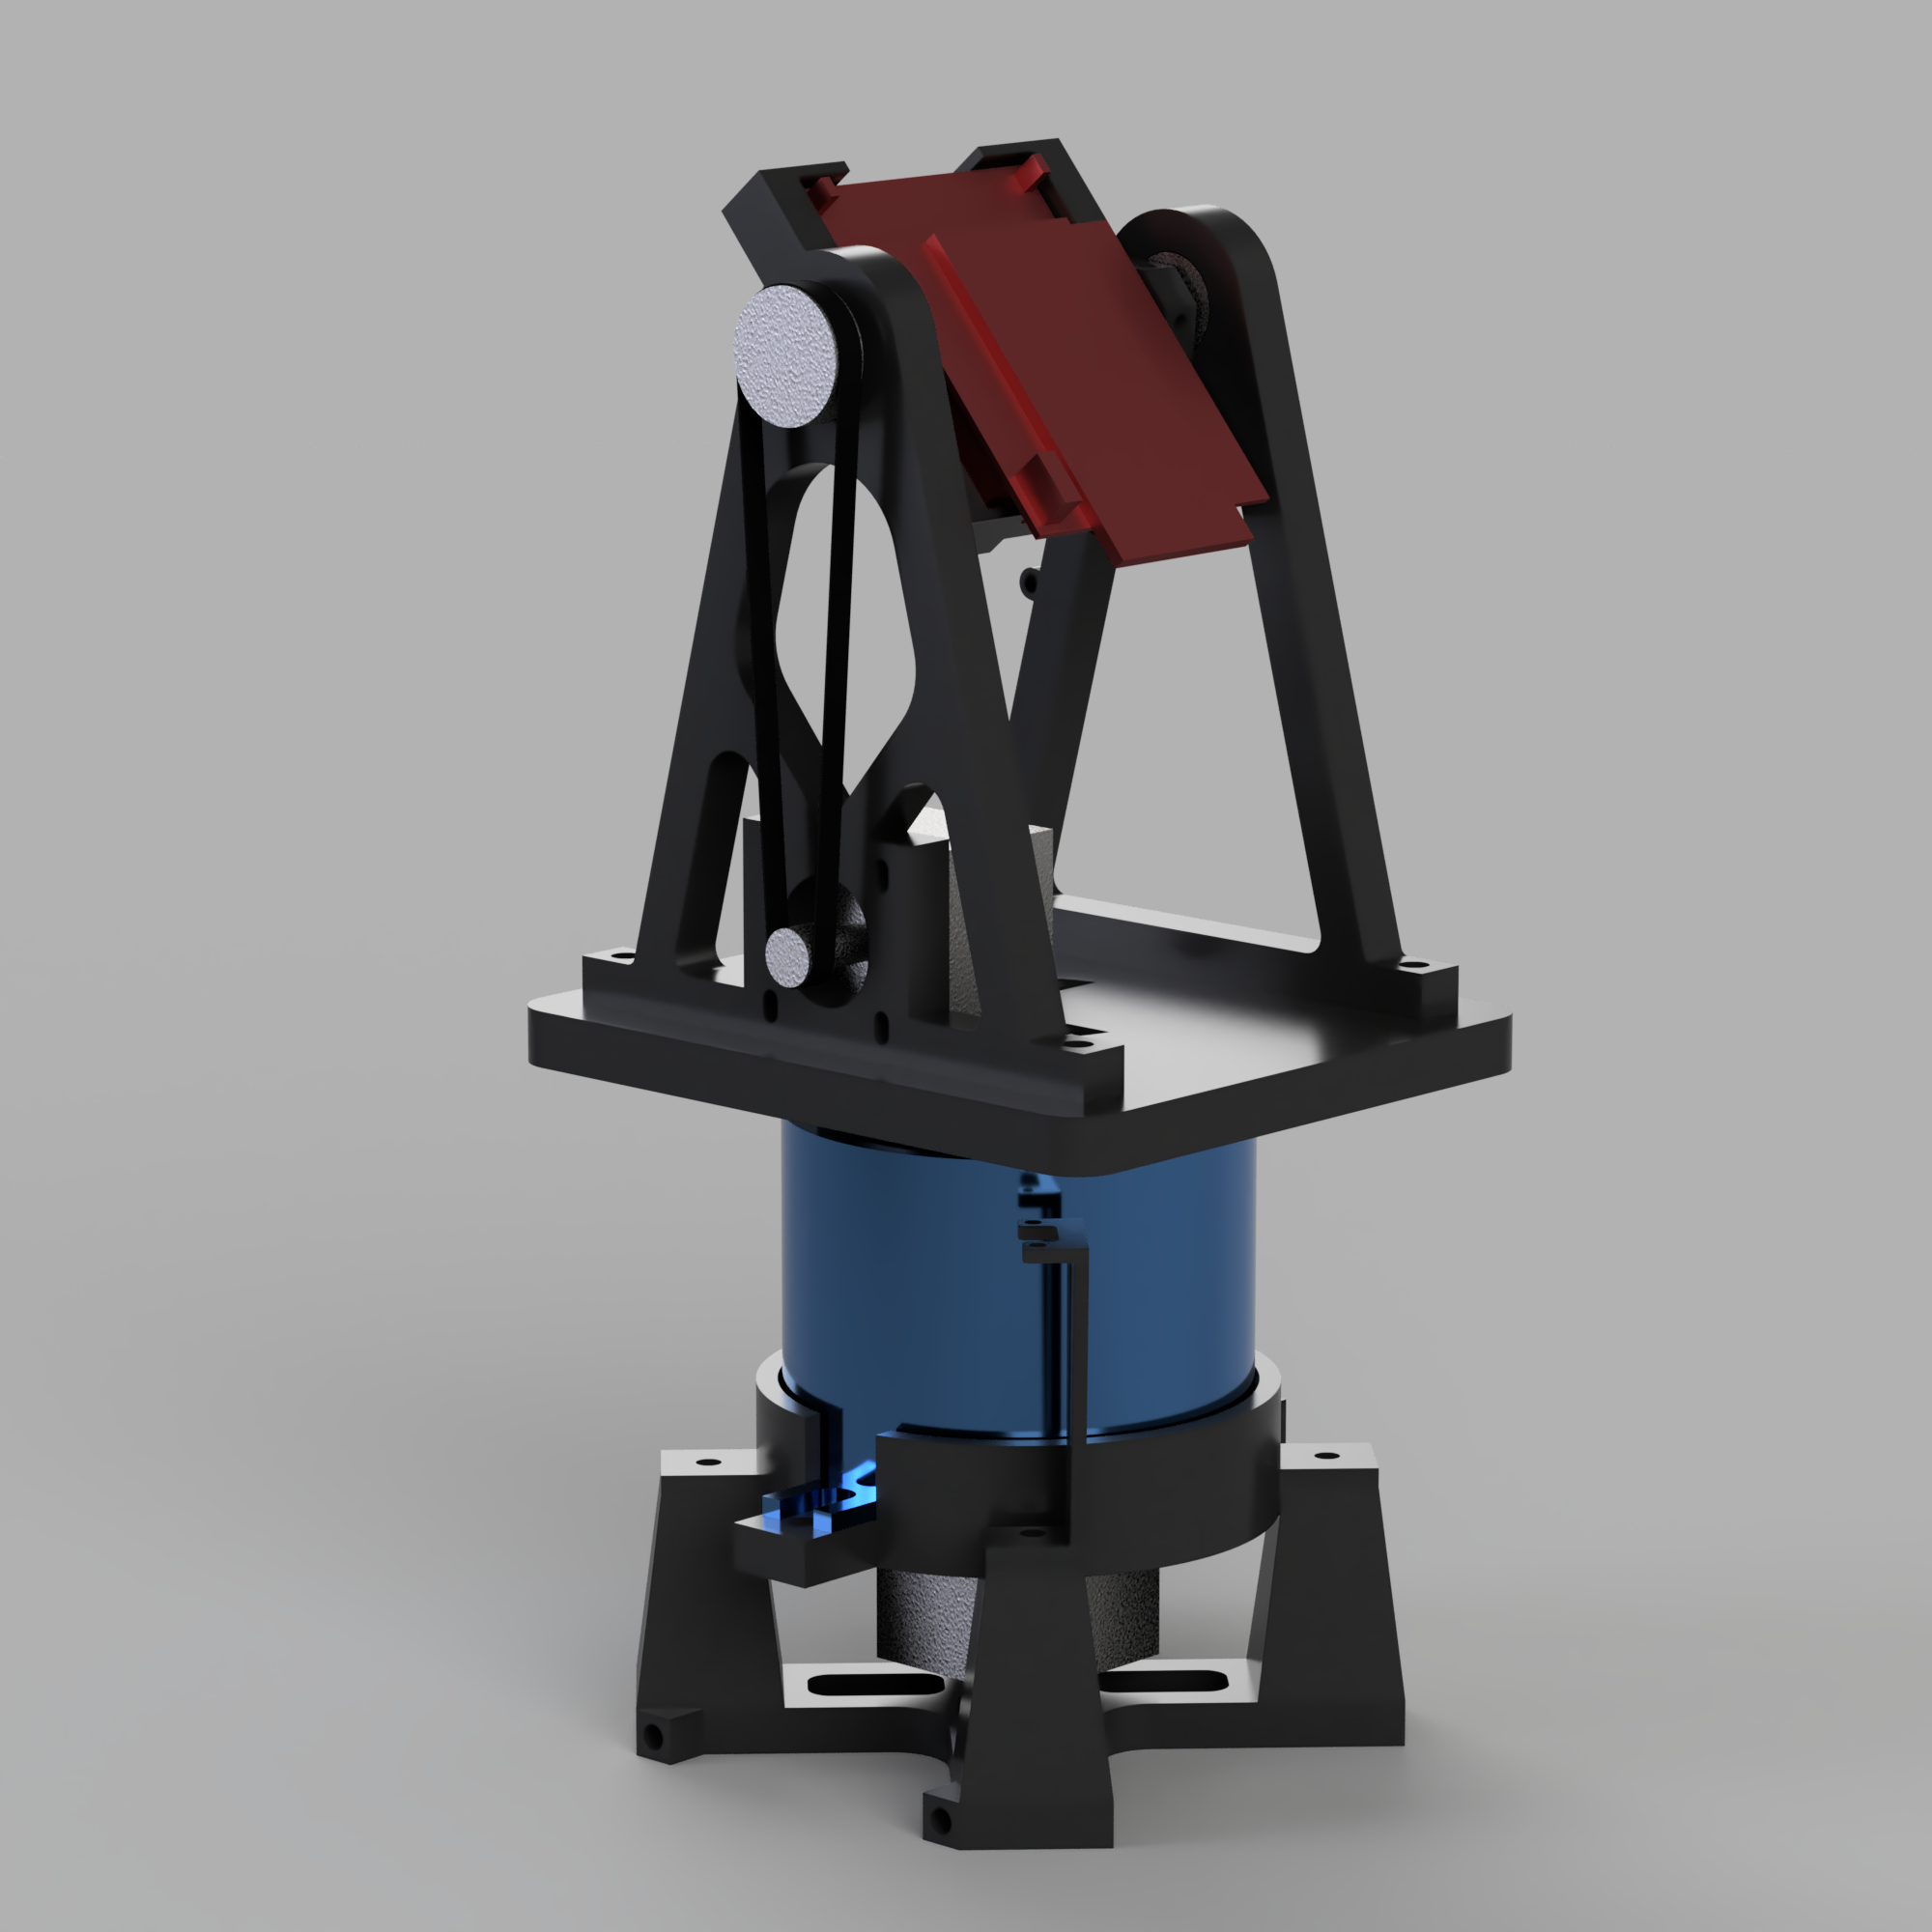
\includegraphics[width=\textwidth]{../img/whole_assembly_2.png} % Replace with your image path
    \caption{3D render}
  \end{subfigure}
  \hspace{0.05\textwidth} % Adjust spacing
  \begin{subfigure}[b]{0.45\textwidth}
    \centering
    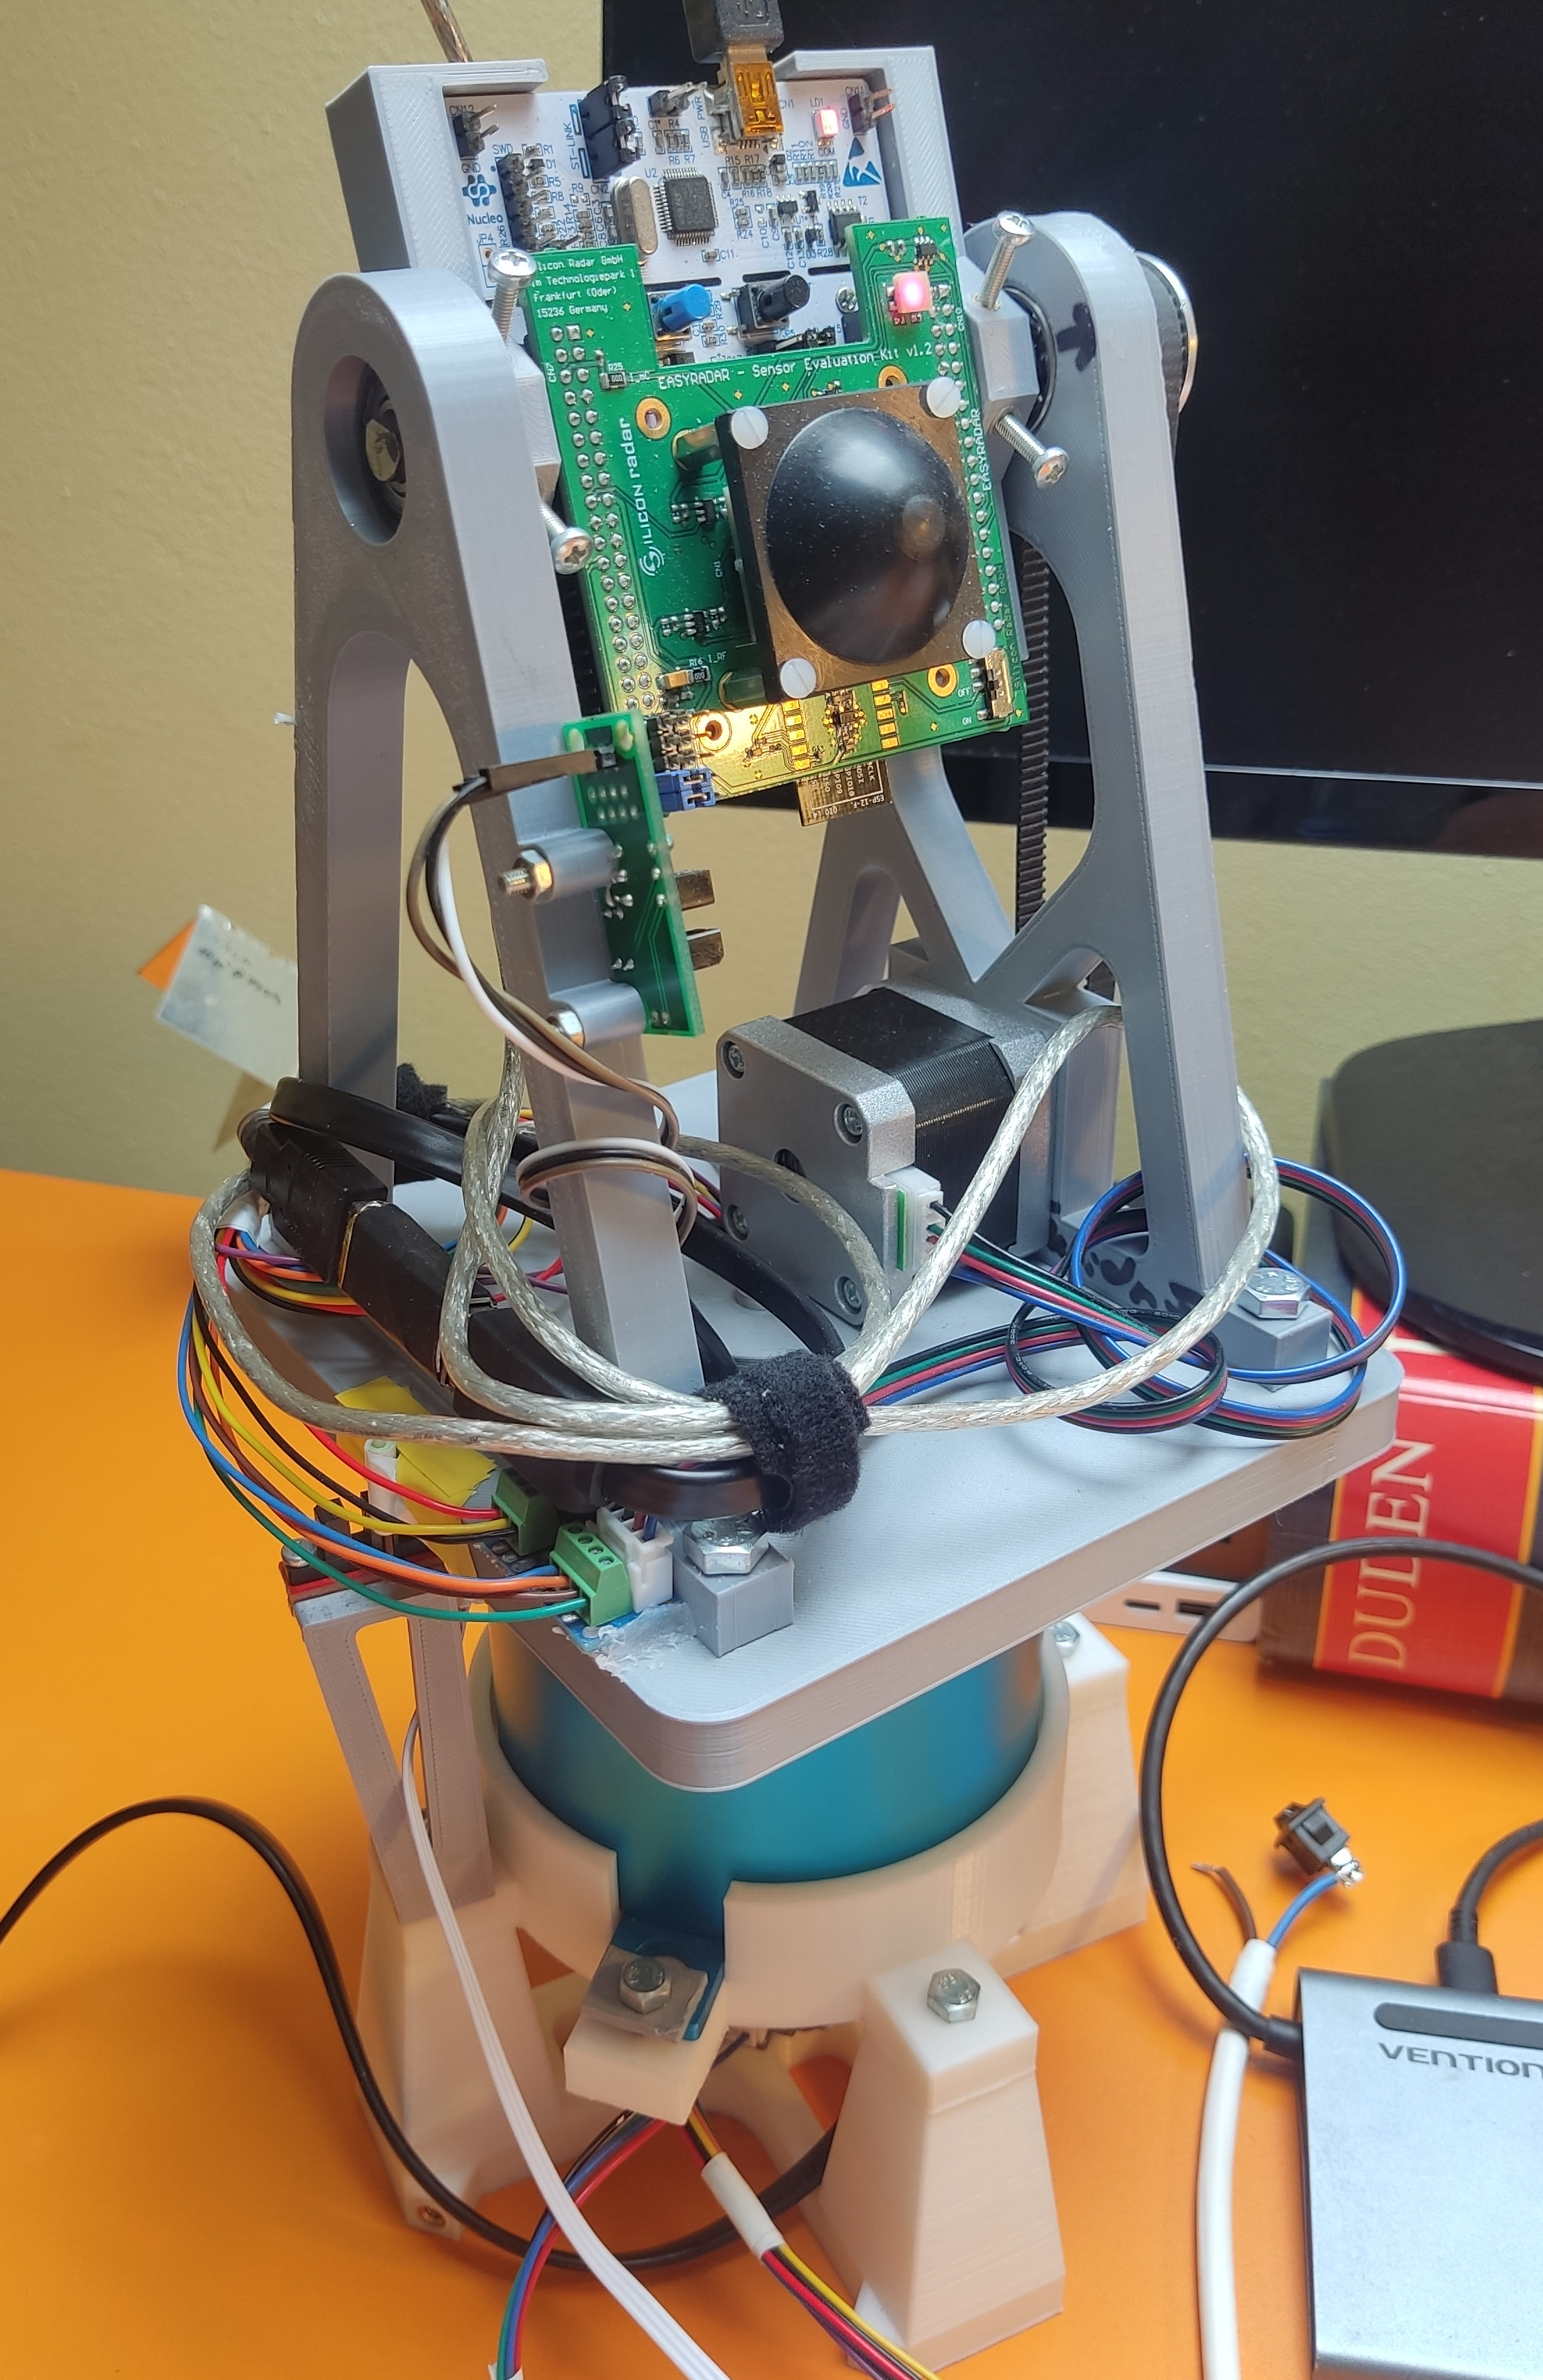
\includegraphics[width=0.75\textwidth]{../img/assembly_photo.jpg} % Replace with your image path
    \caption{Photo}
  \end{subfigure}
  \caption{Form of the final assembly}
  \label{fig:side_by_side}
\end{figure}

\section{Electronics}

Electronic side of the project is rather simple given that only control of two stepper motors and having ability to home their position is needed.
The system is managed by an ESP32 microcontroller. Since the project does not demand advanced capabilities, a basic ESP32 model is sufficient.

Given the low load on the stepper motors and the platform's inability to accumulate significant momentum, a simple stepper driver without feedback control is adequate.
For this purpose, the A4988 stepper driver given its low cost, microstepping capabilities and basic current control\cite{a4988} was selected..

To implement homing, two potential solutions were considered: Hall effect sensors and optical gates.
While Hall effect sensors offer the advantage of angle sensing, allowing correction of any positional drift during operation, they require precise alignment.
Since if the orthogonal Hall effect sensor is not perfectly placed in the axis of rotation, calibration becomes necessary \cite{hall}.

For simplicity and ease of integration, optical gates were selected to enable homing.
This decision eliminates the need for complex calibration while providing reliable functionality.


\chapter{Software realization}

To maximize efficiency in processing commands and ensure accurate stepper motor control, the program workflow is divided into three distinct layers, as illustrated in Figure \ref{fig:code_diag}.

The commonly used two-component architecture—where one component handles communication/command parsing and the other manages execution—was deemed unsuitable for this use case.
Such an approach would complicate integration of programming interface and require just-in-time processing of commands, which could lead to performance issues.

In the chosen architecture, the degree of abstraction decreases with each successive layer, simplifying processing at each step.
This design allows the final layer to operate with maximum efficiency, where transitioning from one command to the next is primarily limited by the inertia of the stepper motors and not by the software.

\begin{figure}[h!]
  \centering


  \begin{tikzpicture}[scale=0.9, node distance=1.5cm]

    % Layer headers
    \node (comm_layer) [layerheader] at (0, 0) {Communication Layer};
    \node (app_layer) [layerheader] at (6, 0) {Application Layer};
    \node (hal_layer) [layerheader] at (12, 0) {HAL Layer};

    % Communication Layer
    \node (comm_start) [startstop, below of=comm_layer, yshift=-0.3cm] {Start};
    \node (wait_serial) [process, below of=comm_start] {Wait for serial data};
    \node (parse_gcode) [process, below of=wait_serial] {Parse G-code};
    \node (parse_success) [decision, below of=parse_gcode, align=center, yshift=-1.3cm] {Parsing\\ Successful?};
    \node (store_command) [process, below of=parse_success, align=center, yshift=-1.8cm] {Store command\\ queue ? program};
    \node (send_response) [process, below of=store_command,yshift=-0.25cm] {Send response};

    % Arrows in Communication Layer
    \draw [arrow] (comm_start) -- (wait_serial);
    \draw [arrow] (wait_serial) -- (parse_gcode);
    \draw [arrow] (parse_gcode) -- (parse_success);
    \draw [arrow] (parse_success.east) -- ++(1, 0) |- (send_response.east) node[midway, left, yshift=+0.25cm] {No};
    \draw [arrow] (parse_success.south) -- ++(0, -0.5) -| (store_command.north) node[midway, right, yshift=+0.05cm] {Yes};
    \draw [arrow] (store_command) -- (send_response);
    \draw [arrow] (send_response.west) -- ++(-0.5, 0) |- (wait_serial.west);

    % Application Layer
    \node (app_start) [startstop, below of=app_layer, yshift=-0.3cm] {Start};
    \node (update_position) [process, below of=app_start] {Update position};
    \node (check_queues) [decision, below of=update_position, yshift=-1.3cm] {Queues full?};
    \node (load) [process, below of=check_queues, align=center, yshift=-1.5cm] {Load command \\ queue ? program};
    \node (process_command) [process, below of=load,yshift=-0.25cm] {Process command};
    \node (store_command) [process, align=center, below of=process_command] {Add command \\ to stepper queue};

    % Arrows in Application Layer
    \draw [arrow] (app_start) -- (update_position);
    \draw [arrow] (update_position) -- (check_queues);
    \draw [arrow] (check_queues.east) -- ++(1, 0) |- (update_position.east) node[midway, left, xshift=0.2cm, yshift=+0.25cm,xshift=0.2cm] {Yes};
    \draw [arrow] (check_queues.south) -- ++(0, -0.5) -| (load.north) node[midway, right, yshift=+0.1cm] {No};
    \draw [arrow] (load.south) -- ++(0, -0.5) -- (process_command.north);
    \draw [arrow] (process_command) -- (store_command);
    \draw [arrow] (store_command.west) -- ++(-0.5, 0) |- (update_position.west);


    \node (hal_start) [startstop, below of=hal_layer, yshift=-0.3cm] {Start};
    \node (wait_queue) [process, below of=hal_start] {Wait on queue};
    \node (execute_command) [process, below of=wait_queue] {Execute command};
    \node (wait_command) [process, below of=execute_command] {Wait on command};
    \node (update_info) [process, align=center, below of=wait_command] {Update last \\command};

    % Arrows in HAL Layer
    \draw [arrow] (hal_start) -- (wait_queue);
    \draw [arrow] (wait_queue) -- (execute_command);
    \draw [arrow] (execute_command) -- (wait_command);
    \draw [arrow] (wait_command) -- (update_info);
    \draw [arrow] (update_info.west) -- ++(-0.5, 0) |- (wait_queue.west);

  \end{tikzpicture}

  \caption[Programm diagram]{Programm diagram}
  \label{fig:code_diag}
\end{figure}

\section{Communication layer}

The communication layer manages incoming data over the serial line, with efficient handling facilitated with the aid of RTOS queues.
Upon receiving data the text string is parsed and either push to queue (if we are declaring a programm) or added to programm declaration.

Immediately after parsing response is send to the user confirming whether the command was parsed correctly or not.
However as communication layer does not a can not check command within context of all previous commands it is possible that command will be parsed correctly but its execution will fail in the application layer.


\section{Application layer}

The application layer performs two primary functions: tracking the current device position and scheduling commands to be sent to the stepper motors.
Aside from tracking current position program also keeps track of the end position of the last scheduled command.
Thanks to this the application layer can handle calculations necessary for absolute positioning and enforce movement limits.

A significant departure from standard G-code interpreters is the platform's handling of single-axis move commands.
If a move command targets only one axis, the other axis remains free to read the next command and begin execution.
If this behavior is undesirable, the user must issue commands for both axes.
In relative positioning mode, a zero value will result in no motion; in absolute positioning mode, the command must specify the current position for no movement to occur.

A key departure from standard G-code interpreters is how the platform handles single-axis move commands.
When a move command targets only one axis, the other axis remains free to read the next command and begin execution.
If this behavior is undesirable, the user must issue commands for both axes.
In relative positioning mode, a zero value results in no motion; in absolute positioning mode, the command must specify the current position to prevent movement.

This behavior is a necessary side effect of the spindle regime, which typically cannot be toggled on or off dynamically.
Another consequence is the requirement for separate positioning modes for each axis.
Continuous rotation prevents the calculation of a move’s end position, making it impossible to pre-schedule absolute positioning commands.




\section{HAL Layer}

The final layer manages stepper motor control and provides the application layer with essential data for position calculations.
In its loop, the program waits for the next command in the stepper queue.
Upon receiving a command, it sets up execution, waits for one or both steppers to complete their movement, and then proceeds to the next command.
Since limit and absolute positioning calculations are handled in the application layer whole routine remains highly efficient.

The main challenge lies in generating precise PWM signals and stopping signal generation after a specific number of steps.
Using the equation:
%
\begin{equation}
  t_{\mathrm{delay}}(s) = \frac{60}{2\cdot N_{\mathrm{steps}} \cdot s},
  \label{eq:delay}
\end{equation}
%
where $s$ is speed in RPM, $N_{\mathrm{steps}}$ is the number of steps, and $t_{\mathrm{delay}}$ is the time between steps, we calculate that even at 30 RPM, the delay between output changes is 5 ms per step.
With microstepping at a 2:1 ratio, this reduces to 2.5 ms -- faster than lowest sleep interval and without sleep watchdog will trigger.
Therefore, signal generation must leverage specialized microcontroller peripherals.

The ESP32 platform offers two options: Remote Controlled Transceiver (RMT) and Motor Control Pulse Width Modulation (MCPWM) combined with Pulse Counter (PCNT).
While RMT allows smooth PWM frequency adjustments, it has several drawbacks.
These include: generating a specific number of pulses is supported only on newer ESP32 models \cite{gitRMT}, synchronization is restricted to its proprietary API, and there is no straightforward way to track progress during a move \cite{espRMT}.

For these reasons, MCPWM and PCNT were chosen.
MCPWM handles pulse generation, while PCNT counts steps, enabling easy synchronization, continuous rotation, and a robust API for step tracking \cite{espPCNT}.
The only limitation is the PCNT’s 15-bit counter, which caps the maximum steps per move at 32,767.


\subsection{Performance of HAL Layer}


Table \ref{tab:performancepwm} illustrates the stability of PWM generation by the MCPWM module at various speeds.
Measurements were conducted using a Saleae Logic Pro 16 logic analyzer, with no microstepping enabled.

The results show that frequency deviation is minimal, though the generated speed is consistently marginally faster than the target, and  the error increases slightly with higher speeds.
Nevertheless, for 24,000 steps at 120 RPM, the relative error in time taken would be only $\epsilon = -0.004\%$, demonstrating excellent accuracy.


\begin{table}[h!]
  \centering
  \caption[Stability of PWM generation]{Stability of PWM generation}
  \begin{tabular}{| m{2cm} || m{2.5cm} | m{2.5cm} | m{2.5cm} | m{2.5cm} |}
    \hline
    RPM & $f_{\mathrm{desired}}$ (Hz) & $f_{\mathrm{low}}$ (Hz) & $f_{\mathrm{high}}$ (Hz) & $f_\mathrm{avg}$ (Hz) \\
    \hline
    10  & 33.334                      & 33.334                  & 33.334                   & 33.334                \\
    30  & 100                         & 100                     & 100.003                  & 100.002               \\
    60  & 200                         & 200                     & 200.01                   & 200.004               \\
    120 & 400                         & 400                     & 400.02                   & 400.007               \\
    \hline
  \end{tabular}
  \label{tab:performancepwm}
\end{table}

\begin{figure}[h!]
	\centering
	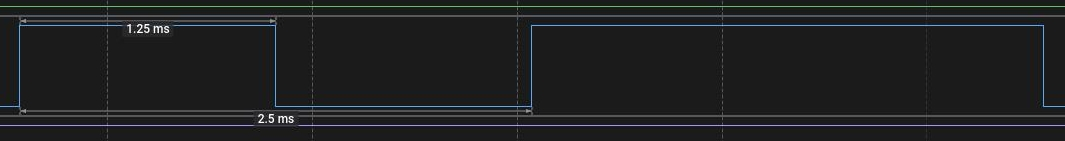
\includegraphics[width=0.7\textwidth]{../img/120rpm_to60_1.jpg}
	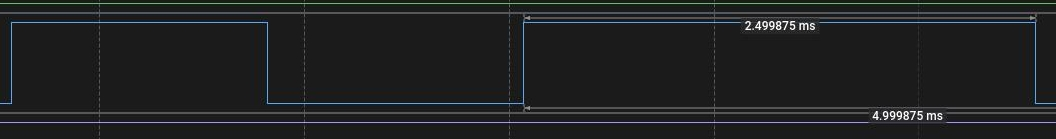
\includegraphics[width=0.7\textwidth]{../img/120rpm_to60_2.jpg}
	\caption[Moment of change between commands with 120RPM and 60RPM]{Moment of change between commands (120RPM $\Rightarrow$  60RPM)}
	\label{fig:switching}
\end{figure}

An attempt was made to measure the speed of switching between commands, as shown in Figure \ref{fig:switching}.
The results indicate that the delay between commands is imperceptible, with similar outcomes observed for other command combinations.

This demonstrates the efficiency of the HAL layer in managing stepper motor control and transitioning seamlessly between commands.
As long as the stepper queues are supplied with commands in advance, the platform can operate without noticeable interruptions.
Most importantly, the platform’s timely and predictable behavior ensures that mathematical corrections to the radar data can be applied accurately.


% RPM & desired  & low interval & high interval & deviation

% speed how fast follow on command gets executed

%% Table how fast are command processed
%% Table with how reliable is timing (with different rpm)

% vim.ft=tex
\chapter*{Conclusion}
\addcontentsline{toc}{chapter}{Conclusion}

TODO


%%% Bibliography (literature used as a source)
%%%
%%% We employ biblatex to construct the bibliography. It processes
%%% citations in the text (e.g., the \cite{...} macro) and looks up
%%% relevant entries in the bibliography.bib file.
%%%
%%% See also biblatex settings in thesis.tex.

%%% Generate the bibliography. Beware that if you cited no works,
%%% the empty list will be omitted completely.

% We let bibliography items stick out of the right margin a little
\def\bibfont{\hfuzz=2pt}

\printbibliography[heading=bibintoc]

%%% If case you prefer to write the bibliography manually (without biblatex),
%%% you can use the following. Please follow the ISO 690 standard and
%%% citation conventions of your field of research.

% \begin{thebibliography}{99}
%
% \bibitem{lamport94}
%   {\sc Lamport,} Leslie.
%   \emph{\LaTeX: A Document Preparation System}.
%   2nd edition.
%   Massachusetts: Addison Wesley, 1994.
%   ISBN 0-201-52983-1.
%
% \end{thebibliography}

% \printbibliography

\listoffigures

\listoftables

\clearpage
\openright
\end{document}
